\section{ETL and Digitisation Layer}

\begin{frame}
    \frametitle{ETL- Components}
    \begin{figure}
        \centering
        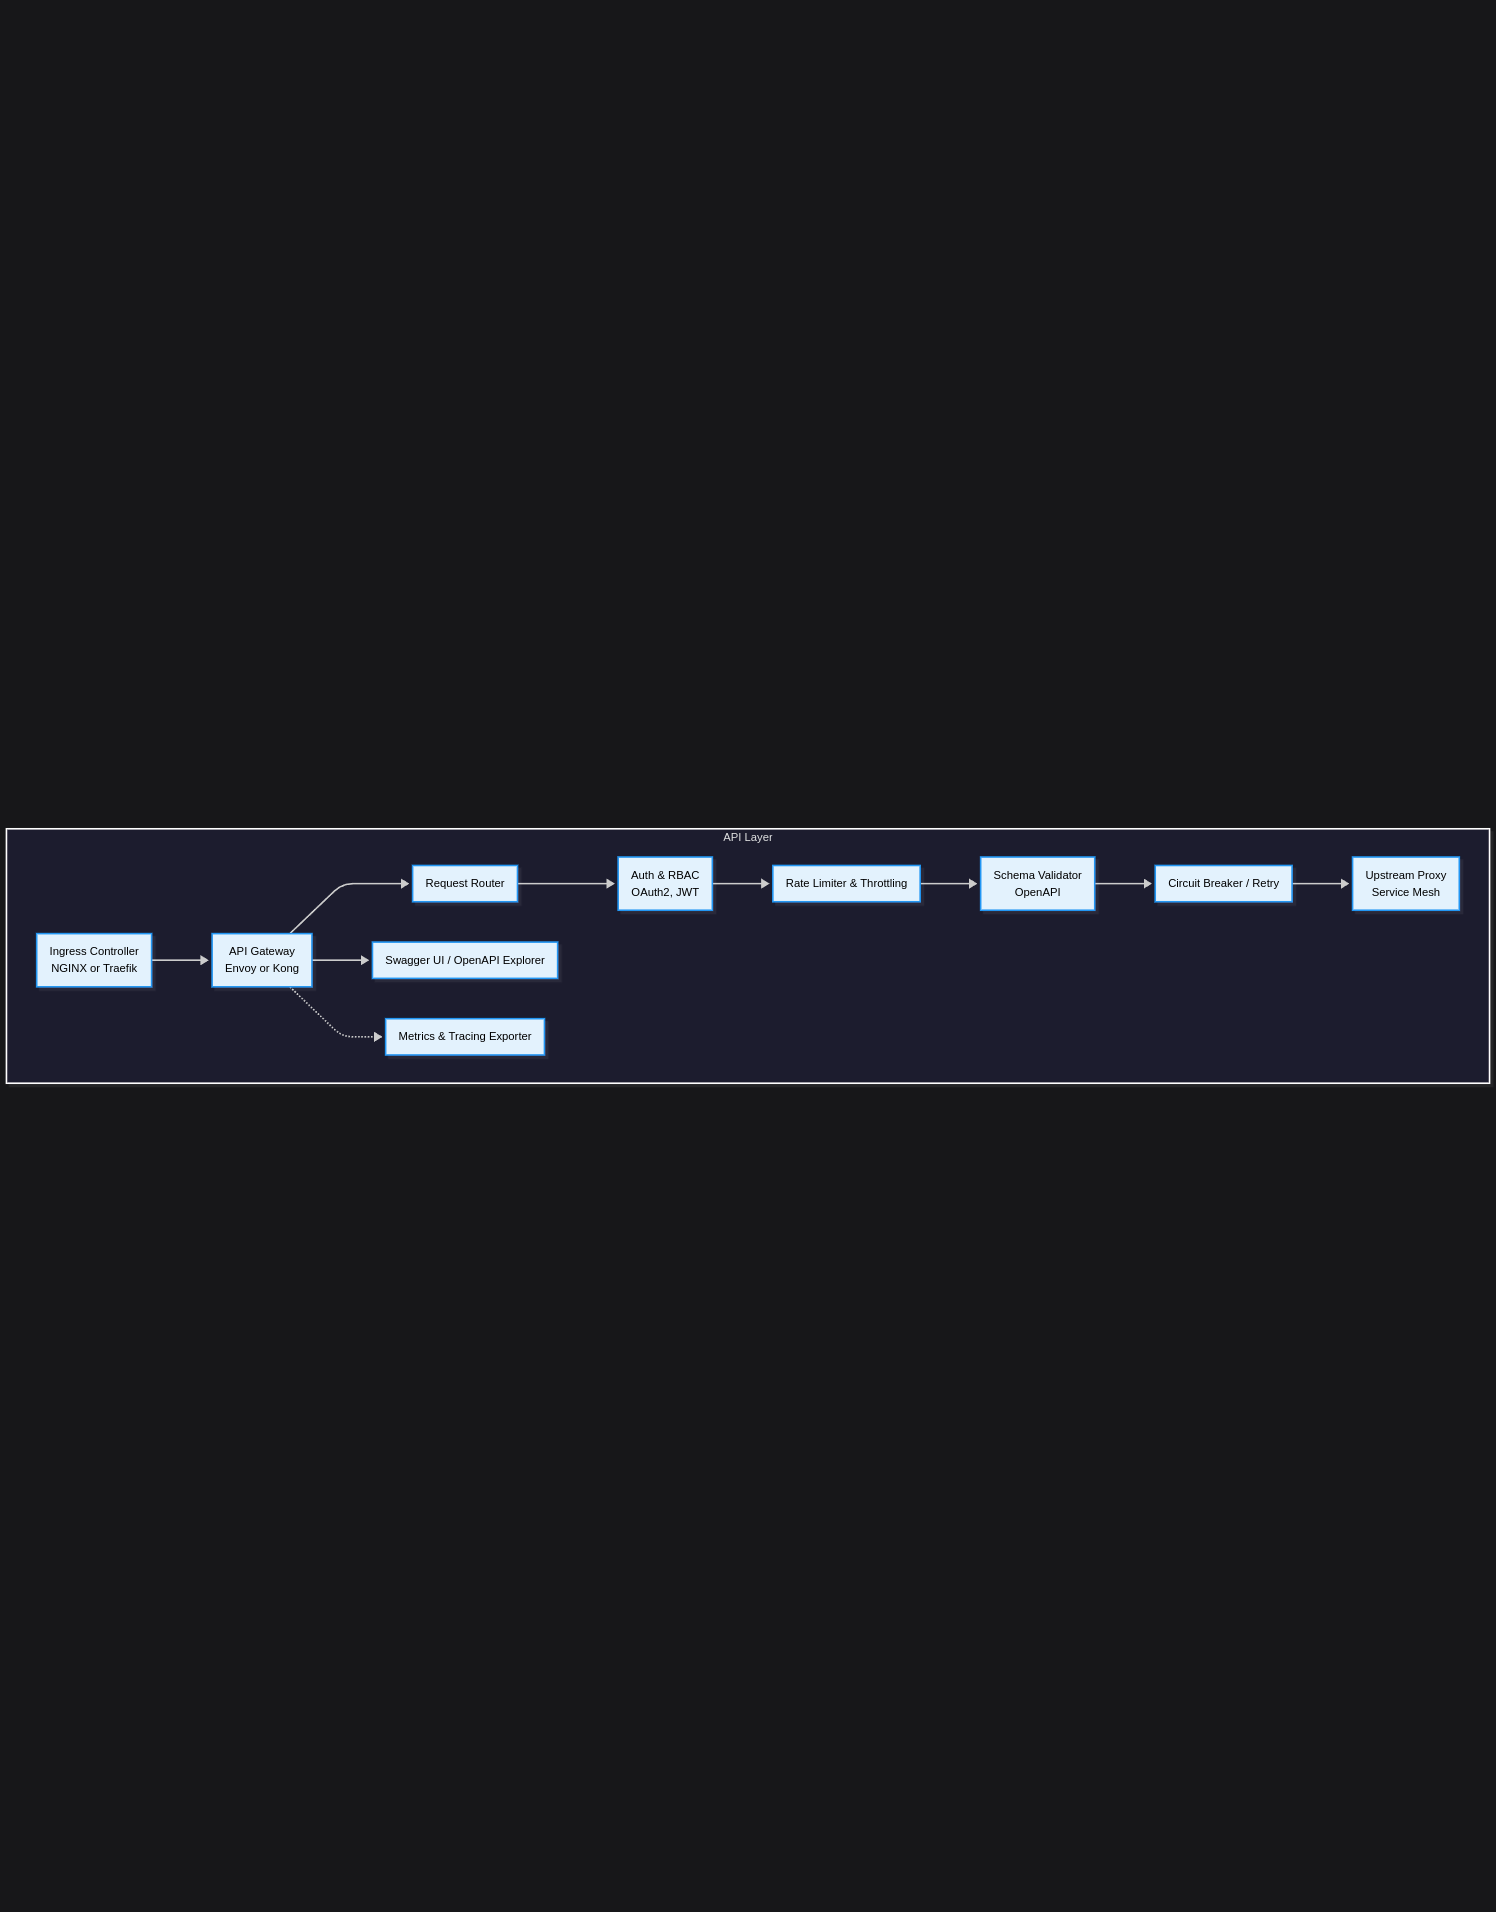
\includegraphics[width=0.8\textwidth]{etl/layout.png} % Adjusted the scale of the image to 0.5
        \caption{ETL Layer Layout}
    \end{figure}
\end{frame}

\begin{frame}
    \frametitle{ETL - Sequence Flow}
    \begin{figure}
        \centering
        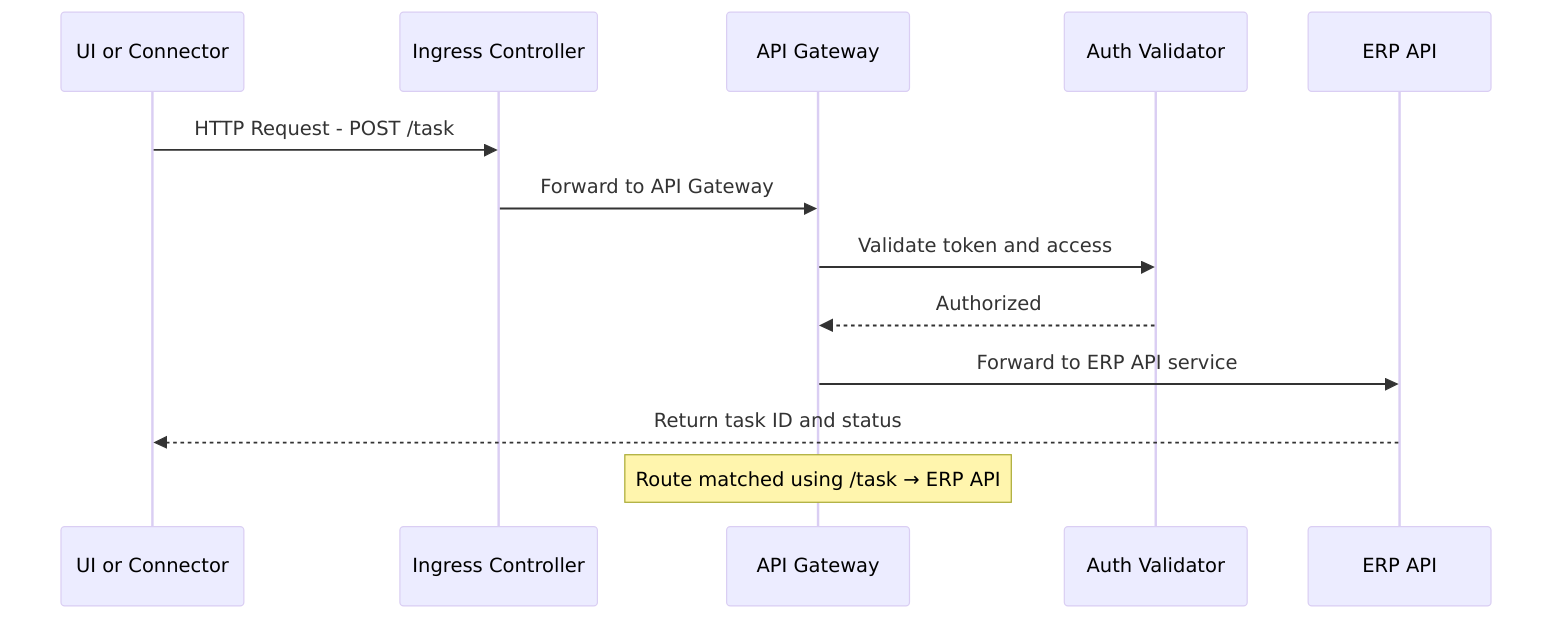
\includegraphics[width=0.8\textwidth]{etl/sequence.png} % Adjusted the scale of the image to 0.5
        \caption{ETL Layer Sequence Flow}
    \end{figure}
\end{frame}



% Dividing the first table into multiple frames with 5 rows each
\begin{frame}
    \frametitle{ETL and Digitisation Layer - Components}
    \begin{itemize}
        \item \textbf{File Watcher}: Detect new files or folder changes from UI or simulation output.
        \item \textbf{Checksum Engine}: Compute hash and compare against existing versions to avoid duplication.
        \item \textbf{Metadata Extractor}: Extract filename, type, timestamp, author, tags.
        \item \textbf{Content Extractor}: Run format-based parsers or OCR tools to extract document content.
        \item \textbf{Simulation Connector}: Pull data from engineering software (e.g., AVEVA, HYSYS) via COM or CLI.
    \end{itemize}
\end{frame}

\begin{frame}
    \frametitle{ETL and Digitisation Layer - Components}
    \begin{itemize}
        \item \textbf{Agent Trigger Manager}: Decide which agents to trigger and when (e.g., document parser, compliance).
        \item \textbf{Error and Retry Handler}: Reattempt failed extractions or flag for manual review.
        \item \textbf{ERP Task Notifier}: Create new ERP tasks or update existing tasks based on file content.
        \item \textbf{Storage Uploader}: Push raw and structured outputs to File Management Layer.
    \end{itemize}
\end{frame}

% % ETL and Digitisation Layer - Technical Responsibilities (Part 1)
% \begin{frame}
%     \frametitle{ETL and Digitisation Layer - Technical Responsibilities (Part 1)}
%     \begin{itemize}
%         \item \textbf{File Watcher}: Uses S3 notifications, Linux inotify, or Windows filesystem events.
%         \item \textbf{Checksum Engine}: Uses SHA-256 or similar to verify content changes.
%         \item \textbf{Metadata Extractor}: YAML/JSON/regex parsers and custom rules per file type.
%         \item \textbf{Content Extractor}: Integrates Tesseract, Donut, PDF parsers, or custom XML/CSV loaders.
%         \item \textbf{Simulation Connector}: Python COM interface via `pywin32`, AutoCAD script runner, HYSYS export tool.
%     \end{itemize}
% \end{frame}

% % ETL and Digitisation Layer - Technical Responsibilities (Part 2)
% \begin{frame}
%     \frametitle{ETL and Digitisation Layer - Technical Responsibilities (Part 2)}
%     \begin{itemize}
%         \item \textbf{Agent Trigger Manager}: Sends API calls or events to AI agent dispatcher per document class.
%         \item \textbf{Error and Retry Handler}: Uses retry queue (e.g., RabbitMQ, Redis) with backoff and alerting.
%         \item \textbf{ERP Task Notifier}: RESTful API call to ERP Task Engine with task context payload.
%         \item \textbf{Storage Uploader}: Calls File Management API to store versioned files and metadata.
%     \end{itemize}
% \end{frame}